\documentclass{ctexart}
\usepackage{xcolor}
\usepackage{setspace}
\usepackage{tikz}
\usepackage{ctex}
\usepackage{geometry}
\usepackage{amsmath}
\usepackage{graphicx} 
\usepackage{subfigure}
\usepackage{float}
\usepackage{algorithm}  
\usepackage{algorithmicx}  
\usepackage{algpseudocode} 
\usepackage{url}
\usepackage{amsthm, amssymb, appendix, bm, graphicx, hyperref, mathrsfs}
\usepackage{tabularx}
\usepackage{booktabs} %需要加载宏包{booktabs}
\usepackage{multirow}
\usepackage{diagbox} % 加载宏包
\usepackage{pifont}

\usepackage{siunitx}
\usepackage{listings}
\usepackage{float}
\pagestyle{plain}

\usetikzlibrary{datavisualization}
\usetikzlibrary{arrows,shapes,chains}
\usepackage{listings}
\lstset{language=C++}
\lstset{breaklines}
\lstset{extendedchars=false}
\lstset{numbers=left}
\geometry{a4paper,left=2.5cm,right=2.5cm,top=2.5cm,bottom=2.5cm}
\CTEXsetup[format={\Large\bfseries\centering}]{section}
\tikzstyle{startstop} = [rectangle,rounded corners, minimum width=3cm,minimum height=1cm,text centered, text width=6cm,draw=black]
\tikzstyle{io} = [trapezium, trapezium left angle = 70,trapezium right angle=110,minimum width=5cm,minimum height=1cm,text centered,draw=black,fill=white]
\tikzstyle{process} = [rectangle,minimum width=3cm,minimum height=1cm,text centered,text width =3cm,text width=6cm,draw=black]
\tikzstyle{decision} = [diamond,minimum width=3cm,minimum height=1cm,text centered,text width=6cm,aspect=2,draw=black,thin]
\tikzstyle{arrow} = [thick,->,>=stealth]
\renewcommand{\algorithmicrequire}{\textbf{Input:}}  % Use Input in the format of Algorithm  
\renewcommand{\algorithmicensure}{\textbf{Output:}} % Use Output in the format of Algorithm  
\newcommand{\subsubsubsection}[1]{\paragraph{#1}\mbox{}\\}
\setcounter{secnumdepth}{4} % how many sectioning levels to assign numbers to
\setcounter{tocdepth}{4} % how many sectioning levels to show in ToC
\begin{document}

\section{模型假设}
1. \quad 基于自身感知的高度信息,本文默认无人机均保持在同一个高度上飞行,即所有无人机在同一个平面上。

2. \quad 假设第一问中的所有小问9架无人机理论上都应均匀分布在半径为100m的圆周上。

3. \quad 假设无人机接收到的方向信息不存在误差。


\subsection{问题一模型的建立与求解}

\subsubsection{极坐标系的建立}

为了更加明确地标注出各编号无人机的标准位置,我们选用包含角度信息的极坐标系来进行刻画。由于被动接收信号的无人机仅能接收到方向信息,即角度,故极坐标系相比直角坐标系更易表达清晰。

假设9架无人机(编号FY01$\sim$FY09)均匀分布在一个半径为100m的圆周上。以编号FY00的无人机作为坐标原点,编号FY00与编号FY01之间的连线作为X轴,建立极坐标系如下图\ref{极坐标系示意图}。各个编号的标准坐标信息如下表:

\begin{figure}[htbp]
  \centering
  \includegraphics[width=0.40\linewidth]{pic/极坐标.jpg}
  \caption{极坐标系示意图}
  \label{极坐标系示意图}
  \end{figure} 

\begin{center}
  表1:各编号无人机标准坐标
  ~\\
    \begin{tabular}{|c|c|c|c|c|c|}
        \hline
        无人机编号&极坐标(m,$^{\circ}$)&无人机编号&极坐标(m,$^{\circ}$)&无人机编号&极坐标(m,$^{\circ}$)\\
        \hline
        FY00&(0,0)&FY01&(100,0)&FY02&(100,40)\\
        \hline
        FY03&(100,80)&FY04&(100,120)&FY05&(100,160)\\
        \hline
        FY06&(100,200)&FY07&(100,240)&FY08&(100,280)\\
        \hline
        FY09&(100,320)& & & &\\    

        \hline
    \end{tabular}\\
\end{center}
\subsubsection{定位模型的建立}
题目要求在已知未知定位无人机与任意两架发射源无人机间连线的夹角后,给出未知定位无人机当前的所在位置。由于发射源无人机的位置是无偏差的,故它们间的距离同样为已知信息。对该问题进行几何分析:

图中A、B、C三点为已知位置的发射源无人机(A为原点,B、C点在圆上按逆时针顺序排列),三点将平面区域划分为4各部分。D点为需要求解的无人机的位置,可能落在任意一个区域中。

其中,A、B和A、C间的距离均为半径r。已知的方向信息包含两个小角与小角组合形成的大角,实际有效信息仅含两个角度。为了方便计算,我们选择包含原点A的角度$\alpha_1$、$\alpha_2$以及发射源无人机间的夹角$\alpha_3$进行分析。

对每个部分的点分别建立定位模型如下:

利用正弦定理及角度关系对$\Delta$ABD,$\Delta$ACD,$\Delta$BCD进行分析,分别列出下列等式:

设$\angle ABD=\theta_1$,$\angle ACD=\theta_2$,$\angle ADB=\alpha_1$,$\angle ADC=\alpha_2$,$\angle BAC=\alpha_3$,AD=l。

(1)若$\alpha_1$、$\alpha_2$之间不存在包含关系,即D点落在I、III区域,分为两种情况讨论:

若D点落在I区域,如图\ref{区域I典型图},则:

\begin{figure}[htbp]
  \centering
  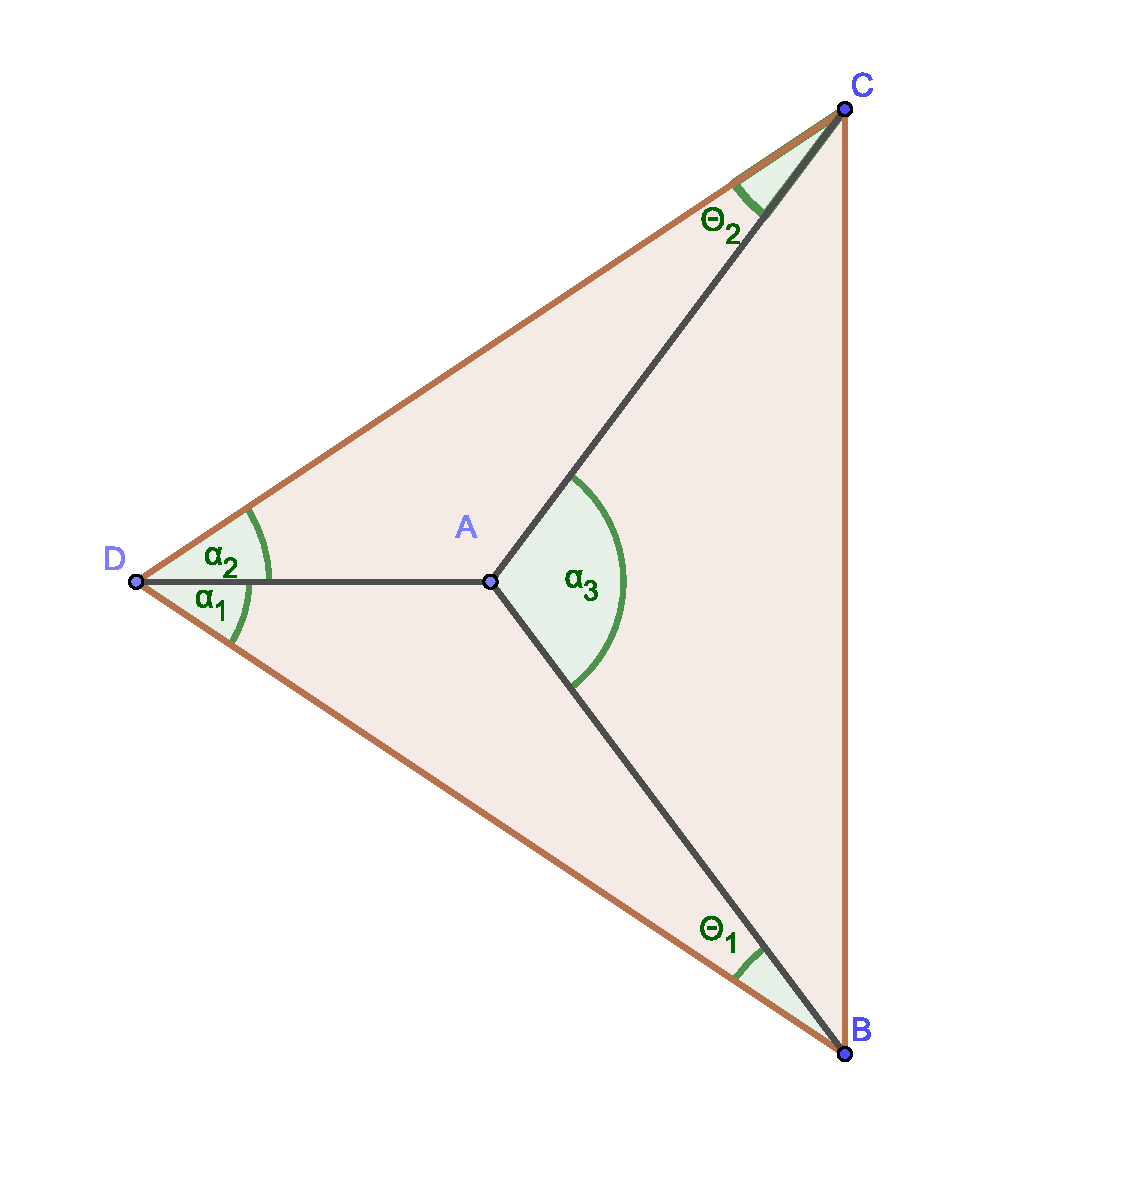
\includegraphics[width=0.40\linewidth]{pic/case1++.eps}
  \caption{区域I典型图}
  \label{区域I典型图}
  \end{figure} 

\begin{equation}
    \left\{
              \begin{array}{ll}
                \theta_1+\theta_2=\alpha_3-(\alpha_1+\alpha_2)=\theta_0\\
                \frac{sin\theta_1}{l}=\frac{sin\alpha_1}{r}=k_1\\
                \frac{sin\theta_2}{l}=\frac{sin\alpha_2}{r}=k_2\\

              \end{array}
            \right.
\end{equation}

\[
    \Rightarrow sin(\theta_0-\theta_1)=\frac{k_2}{k_1}sin\theta_1
\]
\[
    \Rightarrow sin\theta_0 \cdot cos\theta_1-cos\theta_0 \cdot sin\theta_1=\frac{k_2}{k_1}sin\theta_1
\]

\[
    \Rightarrow \theta_1=arctan(\frac{sin\theta_0}{\frac{sin\alpha_2}{sin\alpha_1}+cos\theta_0}),\theta_0=\alpha_3-(\alpha_1+\alpha_2)
\]

在求解过程中,如果发现等式无法计算或出现正无穷的情况,则考虑$\theta_1=90^{\circ}$。

若B的极坐标为(100,$\beta$),则该种情况下,未知点的定位坐标为(100$\times\frac{sin\theta_1}{sin\alpha_1}$,$\beta -$($\pi$-$\theta_1$-$\alpha_1$))。



若D点落在III区域,如图\ref{区域III典型图},则:

\begin{figure}[htbp]
  \centering
  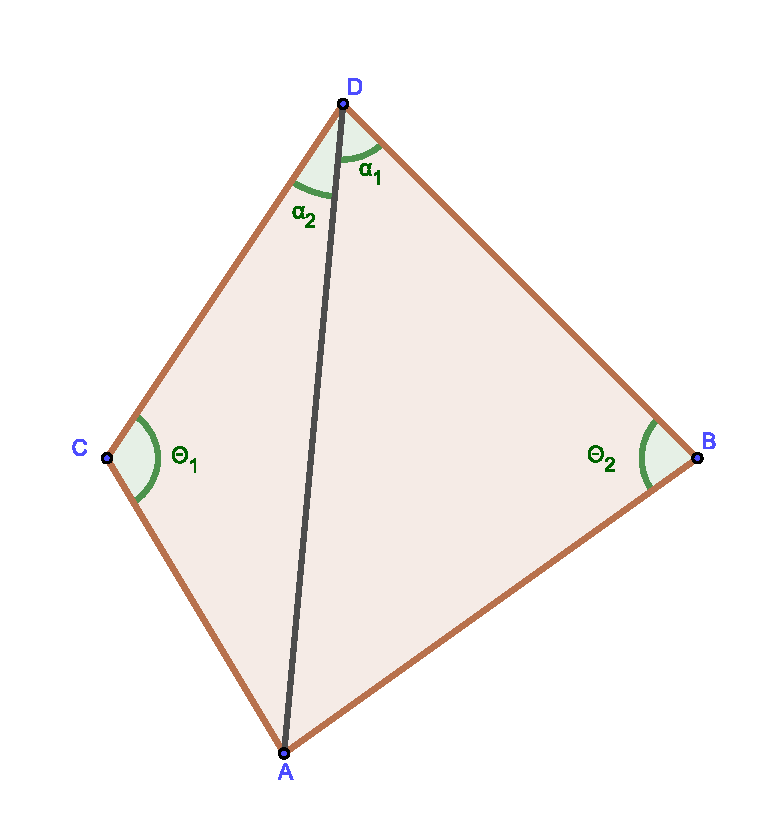
\includegraphics[width=0.40\linewidth]{pic/case3+.eps}
  \caption{区域III典型图}
  \label{区域III典型图}
  \end{figure} 


无论D点在$\Delta ABC$内部还是外部,所建立的方程保持不变。

\begin{equation}
    \left\{
              \begin{array}{ll}
                \theta_1+\theta_2=2\pi-(\alpha_1+\alpha_2+\alpha_3)\\
                \frac{sin\theta_1}{l}=\frac{sin\alpha_1}{r}=k_1\\
                \frac{sin\theta_2}{l}=\frac{sin\alpha_2}{r}=k_2\\

              \end{array}
            \right.
\end{equation}
\[
    \Rightarrow \theta_1=arctan \frac{-sin(\alpha_1+\alpha_2+\alpha_3)}{\frac{sin\alpha_2}{sin\alpha_1}+cos(\alpha_1+\alpha_2+\alpha_3)}
\]
或$\theta_1=90^{\circ}$。

若B的极坐标为(100,$\beta$),则该种情况下,未知点的定位坐标为(100$\times\frac{sin\theta_1}{sin\alpha_1}$,$\beta +$($\pi$-$\theta_1$-$\alpha_1$))。


(2)若$\alpha_1$、$\alpha_2$之间存在包含关系,即D点落在II、IV区域,两种可能性如图\ref{区域II典型图}\ref{区域IV典型图}所示;

\begin{figure}[htbp]
  \begin{minipage}[t]{0.45\linewidth}
  \centering
  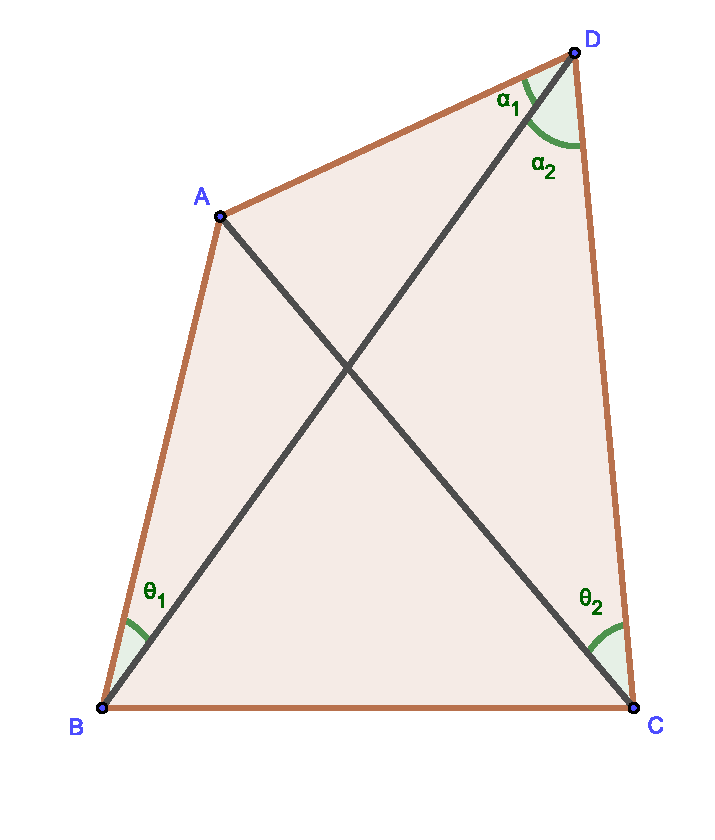
\includegraphics[height=5.5cm,width=5.5cm]{pic/case4.eps}
  \caption{区域II典型图}
  \label{区域II典型图}
  \end{minipage}%
  \begin{minipage}[t]{0.45\linewidth}
  \centering
  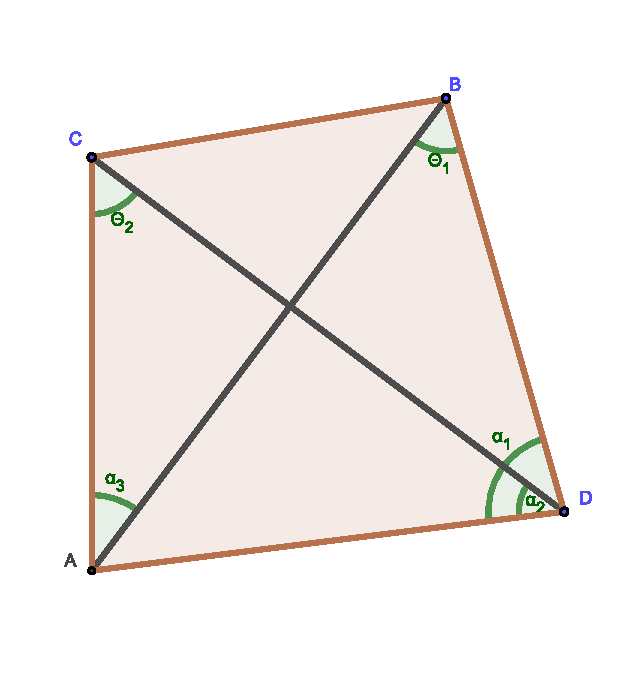
\includegraphics[height=5.5cm,width=5.5cm]{pic/case2+.eps}
  \caption{区域IV典型图}
  \label{区域IV典型图}
  \end{minipage}
  \end{figure}


当$\alpha_1 < \alpha_2$时:

\begin{equation}
    \left\{
              \begin{array}{ll}
                \theta_1-\theta_2=\alpha_2-(\alpha_1+\alpha_3)=\theta_0\\
                \frac{sin\theta_1}{l}=\frac{sin\alpha_1}{r}=k_1\\
                \frac{sin\theta_2}{l}=\frac{sin\alpha_2}{r}=k_2\\

              \end{array}
            \right.
\end{equation}

\[
    \Rightarrow \theta_1=arctan\frac{sin\theta_0}{cos\theta_0-\frac{sin\alpha_2}{sin\alpha_1}},\theta_0=\alpha_2-(\alpha_1+\alpha_3)
\]
或$\theta_1=90^{\circ}$。

若B的极坐标为(100,$\beta$),则该种情况下,未知点的定位坐标为(100$\times\frac{sin\theta_1}{sin\alpha_1}$,$\beta +$($\pi$-$\theta_1$-$\alpha_1$))。


当$\alpha_1 > \alpha_2$时:

\begin{equation}
    \left\{
              \begin{array}{ll}
                \theta_2-\theta_1=\alpha_1-(\alpha_2+\alpha_3)=\theta_0\\
                \frac{sin\theta_1}{l}={sin\alpha_1}{r}=k_1\\
                \frac{sin\theta_2}{l}={sin\alpha_2}{r}=k_2\\

              \end{array}
            \right.
\end{equation}

\[
    \Rightarrow \theta_1=arctan\frac{sin\theta_0}{\frac{sin\alpha_2}{sin\alpha_1}-cos\theta_0},\theta_0=\alpha_1-(\alpha_2+\alpha_3)
\]
或$\theta_1=90^{\circ}$。

若B的极坐标为(100,$\beta$),则该种情况下,未知点的定位坐标为(100$\times\frac{sin\theta_1}{sin\alpha_1}$,$\beta -$($\pi$-$\theta_1$-$\alpha_1$))。

由于$\theta_1$有四种不同的表达方式,故未知点仍有四个可能的坐标位置。 

\subsubsubsection{最终位置的确定}

由于我们无从知道D点究竟落在哪个区域,故四个点的坐标均有可能。然而题目中提及被动接收信号无人机所在位置仅略有偏差,故我们考虑将求解出来的四个坐标分别与标准坐标求欧几里得距离,将其中距离最短的点作为该无人机所在的位置。

距离公式计算方式如下:

设D点的标准坐标为(100,$\gamma_0$),求解出来的其中一个坐标为(100$\times\frac{sin\theta_1}{sin\alpha_1}$,$\beta \pm$($\pi$-$\theta_1$-$\alpha_1$)),则:

\[
 s=\sqrt{100^2+(100\times\frac{sin\theta_1}{sin\alpha_1})^2-2\times100\times(100\times\frac{sin\theta_1}{sin\alpha_1})\times cos(\gamma_0-\beta \pm(\pi-\theta_1-\alpha_1))}
\]

\subsubsection{几何模型的相关检验}

为了验证该位置确定方式的严谨性,我们进行了相关数据的模拟。随机选取两个编号的无人机作为发射源无人机,另外七个编号的无人机k'l作随机扰动,使其略微偏离标准位置。由于我们采用的为极坐标系,所以给出一个扇形区域的误差限,但为了跟实际情况更加匹配,通过调整极径和幅角,使扇形区域尽可能接近方形区域。

经过相关计算,我们给出极径误差为$\pm 5m $,幅角误差为$\pm 3^{\circ}$,从而使得随机误差在10\%以内,且浮动区域约为一个方形,如图\ref{误差范围示意图}所示。

\begin{figure}[htbp]
  \centering
  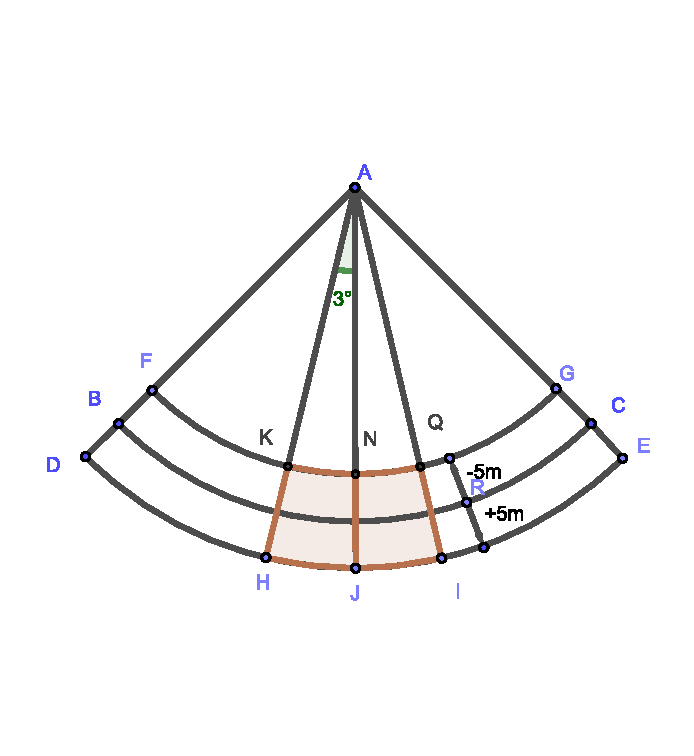
\includegraphics[width=0.45\linewidth]{pic/error area.eps}
  \caption{误差范围示意图}
  \label{误差范围示意图}
  \end{figure}

模拟方式为在9个编号点中选取其中3个,两个点为发射点,一个点为接收点,给接收点设置一个随机扰动,得到一组模拟真实数据。计算接收点与发射源间的方向信息后,将其作为输入,用上文所建的模型进行求解后,得到一组求解数据。用模拟真实数据与求解数据进行比较,以此判断模型的准确性。

选取方案总共有$\begin{pmatrix} 3 \\ 9 \end{pmatrix}\times 3=252$种,将其全模拟并且在随机扰动十万次后,发现模拟真实数据与求解数据间的误差在小数点10位之后,考虑为机器误差。由于数据量过大,故不将具体数据放入正文及附录中,具体内容可见于支撑材料。

\subsubsection{发射源的选取}

共有四类发射源的选取方式,分别与原点的夹角为$\pm 40^{\circ}$,$\pm 80^{\circ}$,$\pm 120^{\circ}$,$\pm 160^{\circ}$。

不断扩大误差范围,直至扩大到误差为30\%(即极径误差限扩大为$\pm 15m$,幅角误差限扩大为$\pm 3^{\circ}$时,出现“报错现象”。“报错现象”的定义为模拟真实位置与求解位置之间的距离超过机器误差eps(根据经验,约为$10^{-8}$)。

在上部分的模拟中,这四类情况我们均有涉及,现为扩大数据量,增加实验可信度,每轮模拟次数调整为10000000次。其中,发射源的圆心角为$40^{\circ}$时,报错概率较小,约为其他几类情况报错概率的$\frac{1}{2}$。

运行三轮的数据基本保持稳定,具体结果如下图\ref{不同发射源圆心角的报错频次图}所示:

\begin{figure}[htbp]
  \centering
  \includegraphics[width=0.75\linewidth]{pic/Rplot01.jpeg}
  \caption{不同发射源圆心角的报错频次图}
  \label{不同发射源圆心角的报错频次图}
  \end{figure}




故在进行发射源的选取时,可以尽可能多考虑圆心角为$40^{\circ}$的两个无人机作为发射源。


\subsection{问题二模型的建立与求解}

在信号源编号未知的情况下,每次多引入一个信号源,只能额外得到以接受信号无人机为顶点的两个有效角度信息。从几何求解角度,其不足以得到定位所需的极径、幅角。于是我们考虑利用已知角度信息先确定至少一架发射信号无人机的编号,即可把该问题等同于问题一,利用相同方法定位。

\subsubsection{角度区间定位模型}
考虑以待定位无人机理想位置为顶点、FY01与另一未知编号无人机所发射信号为两边形成的圆周角,圆周上相邻的发射信号无人机对应的该角度有$20^{\circ}$的变化量。鉴于待定位无人机位置只是略有偏差,故不同发射信号无人机对应的该角度也只是相对理想圆周角略有改变,不同的信号源无人机形成的圆周角仍可认为处于不同的跨度为$20^{\circ}$的角度区间中。

对待定位无人机,根据每$20^{\circ}$对应一个信号来源无人机,对接受到的信号的角度进行线性区间划分。再根据实际测得的角度信息落入的角度区间,找到其对应的发射信号无人机,即可推定信号源无人机的编号。

又由于等长的弦对应的圆周角相等,故由上会得到两个关于过FY01的径向对称分布的均满足该角度情况的信号源无人机编号。

例如在FY04作为待定位无人机、FY03作为一发射信号无人机的情况下,接受到的信号近似圆周角为$38^{\circ}$,此时对各个不同信号源无人机位置,有对应角度划分区间如下表;

\begin{center}
  表2:各编号无人机作信号源时对应角度区间
  ~\\
    \begin{tabular}{|c|c|c|c|c|c|}
        \hline
        无人机编号&角度区间($^{\circ}$)&无人机编号&角度区间($^{\circ}$)&无人机编号&角度区间($^{\circ}$)\\
        \hline
        FY02&[0,30)&FY03&[30,50)&FY05&[70,90]\\
        \hline
        FY06&[70,90]&FY07&[50,70)&FY08&[30,50)\\
        \hline
        FY09&[0,30)& & & &\\    
        \hline
    \end{tabular}\\
\end{center}

该表由FY01作为起始零度点,向两侧每隔$20^{\circ}$进行划分得到。其中因为FY01作为已知的固定发射源存在,故将较小的角度区间直接划分给两侧的FY01、FY09。同时我们将可能的测得角为钝角情况考虑为一对优弧、劣弧对应的一对对称无人机情况,故表中直接考虑其补角即可。

在该情境下,测得的$38^{\circ}$落在了$[30,50)$划分区间,故由表可知其最可能的信号发射来源为FY03、FY08这一对无人机。

\begin{figure}[htbp]
  \centering
  \includegraphics[height=5.5cm,width=5.5cm]{pic/example_for_2.a.jpg}
  \caption{接收信号角度示意图}
  \end{figure}

\subsubsubsection{角度范围划定}

\subsubsubsection{对称点的判断}

当将获得的方向信息对应在相应的角度区间上时,我们可以判断未知发射源无人机的可能编号。编号的可能性一般有两种且关于FY01号无人机的位置对称,为了判别发射源无人机的真实编号,我们对其进行机理分析。

设需要判别的两个编号为$c_1$,$c_2$,其中$c_1+c_2=11$,在圆周上均匀分布着9个点,1个点为已知发射源FY01,2个点为可能发射源。这三个点上无人机的位置不存在偏差,根据对称特性,2个可能发射源与FY01中相隔点的数量相同,将这些相隔点定义为区内点。除去这三类点后,圆周上一定还存在偶数个点,并将这些点定义为区外点,具体定义如下图\ref{点的定义图}。接收信号的无人机的真实位置与这些点略有偏差。

\begin{figure}[htbp]
  \centering
  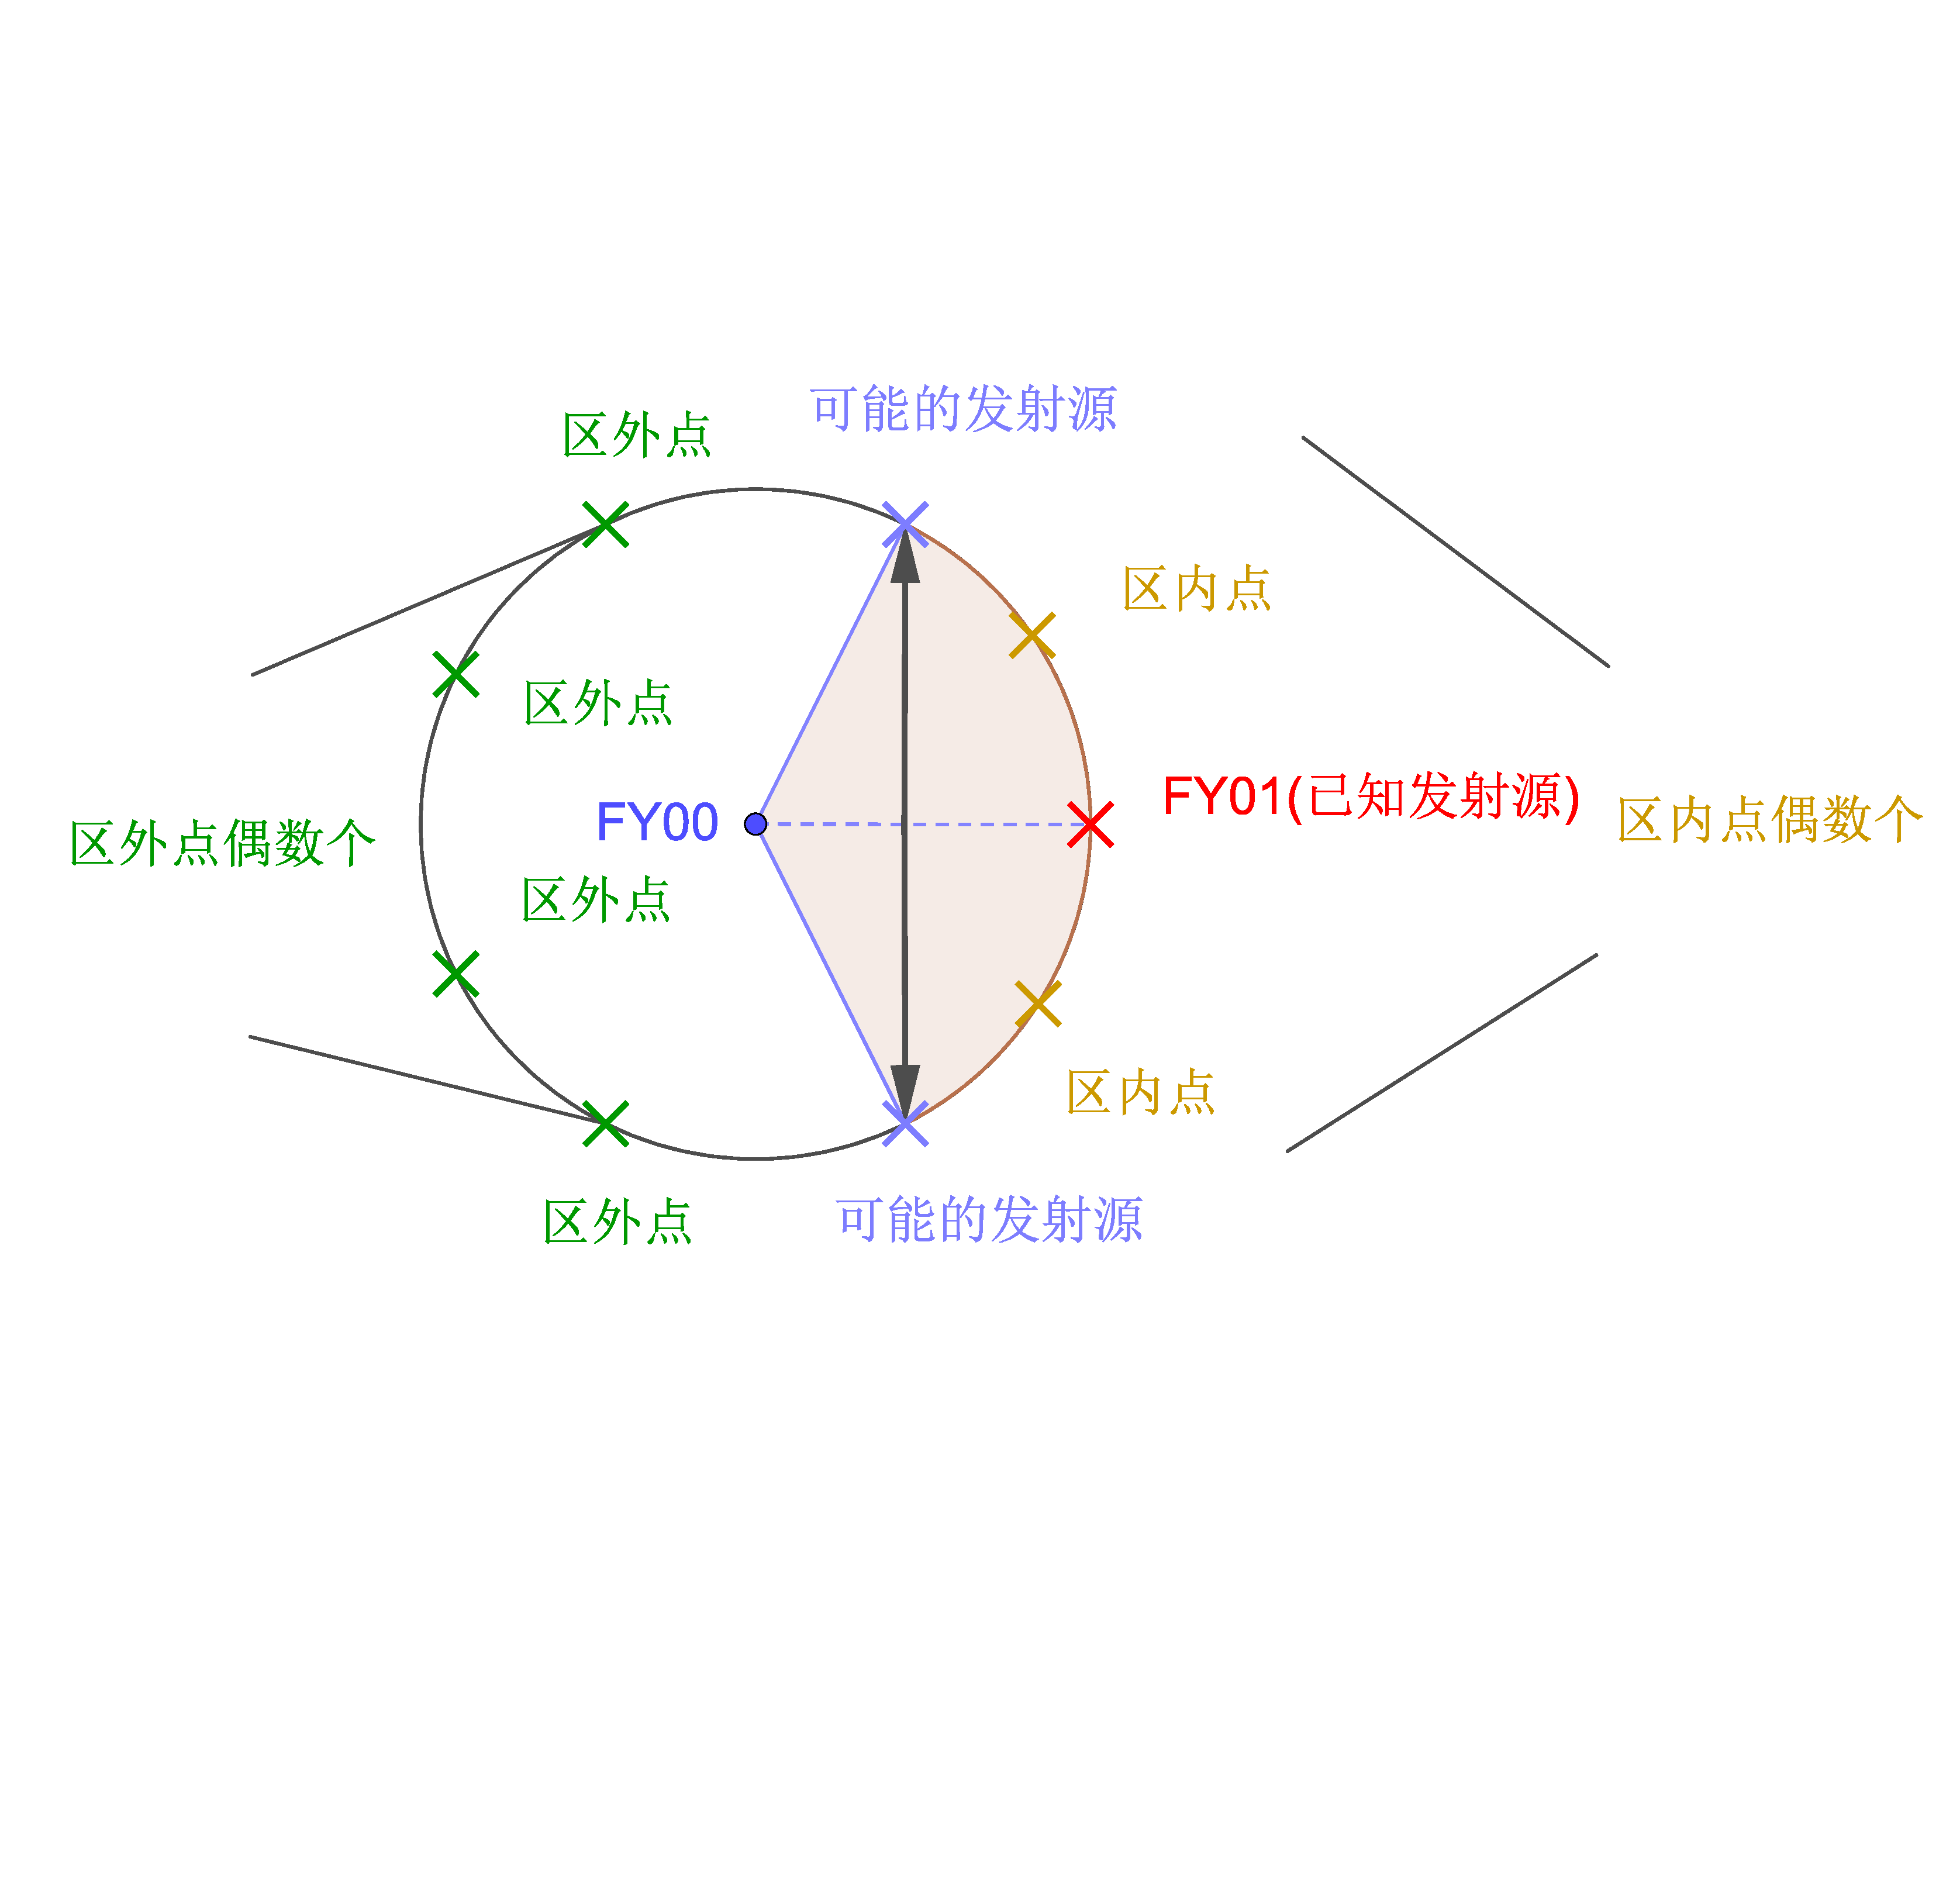
\includegraphics[width=0.75\linewidth]{pic/regional_points.eps}
  \caption{点的定义图}
  \label{点的定义图}
  \end{figure}


接收点存在的位置有两种可能,一种为区内点附近,一种为区外点附近。

为了更清晰地进行阐释,下面给出了两个典型情况的举例(左图为接收点在区内点附近,右图为接收点在区外点附近)。设接收点为FY02/FY06附近略有偏差的点,可能发射源为FY03和FY08。令FY00所在点为O,FY01为P,可能发射源分别为$F_1$、$F_2$,接收点为J,如下图\ref{区内点情况}\ref{区外点情况}所示。

\begin{figure}[htbp]
  \begin{minipage}[t]{0.45\linewidth}
  \centering
  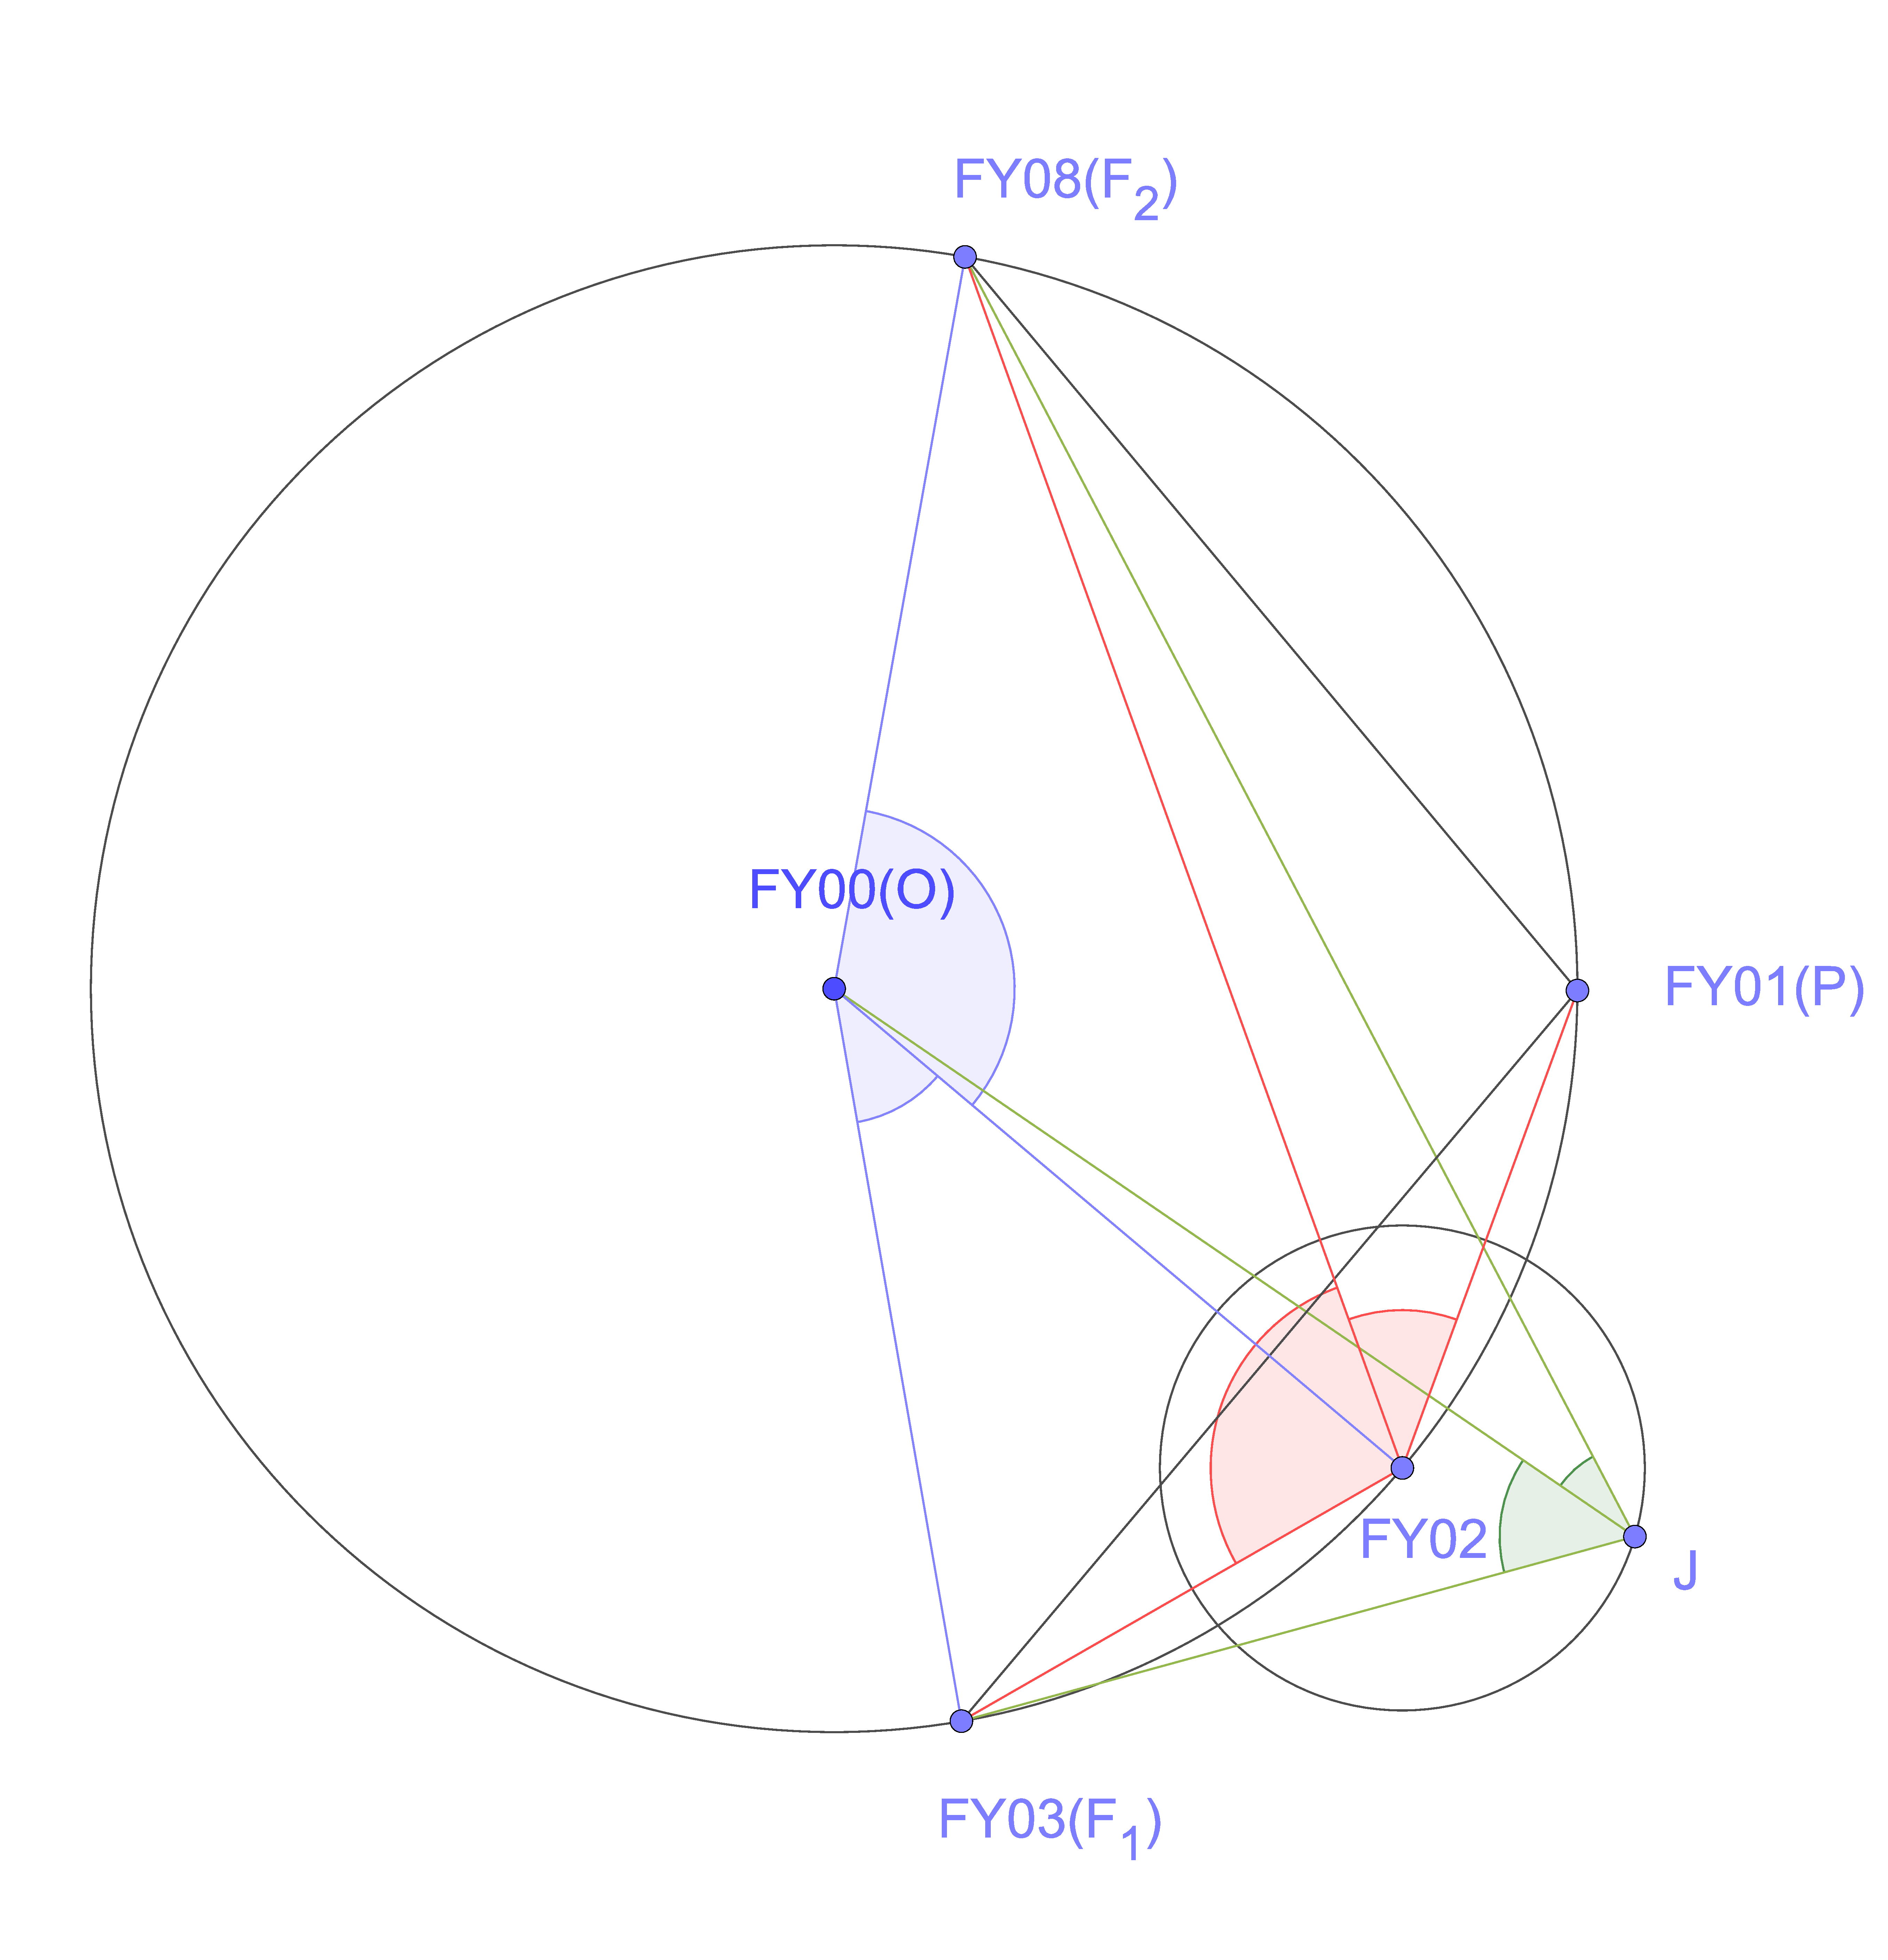
\includegraphics[height=5.5cm,width=5.5cm]{pic/error_circle1(1).eps}
  \caption{区内点情况}
  \label{区内点情况}
  \end{minipage}%
  \begin{minipage}[t]{0.45\linewidth}
  \centering
  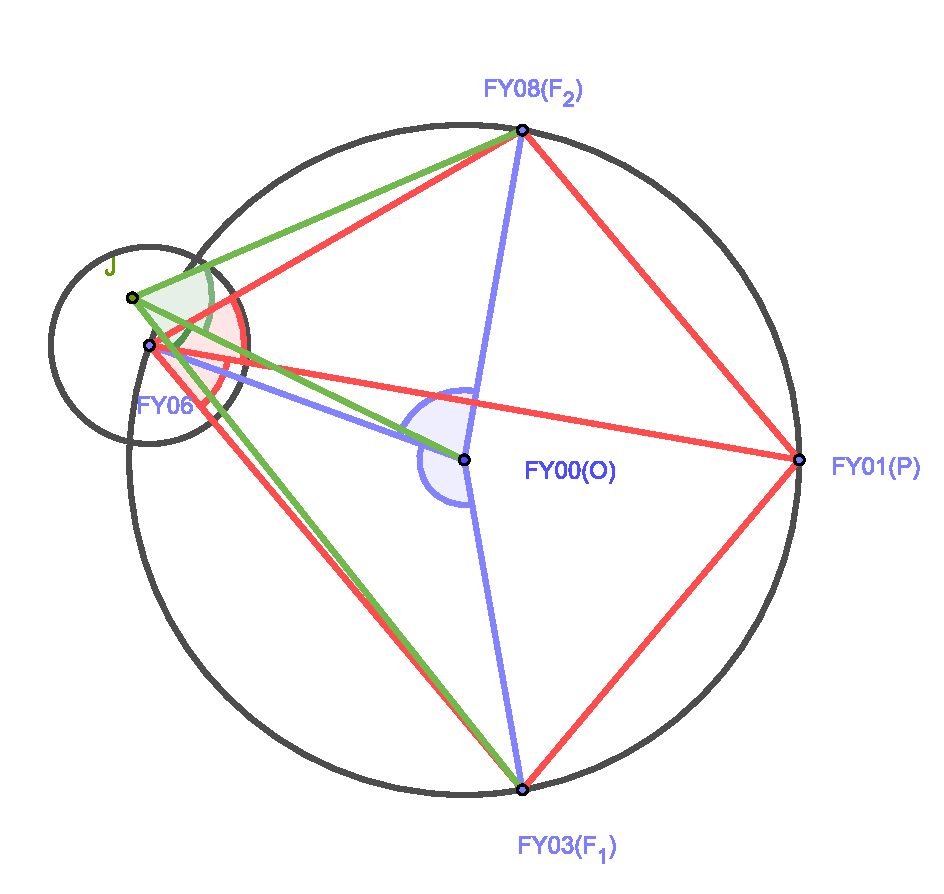
\includegraphics[height=5.5cm,width=5.5cm]{pic/error_circle2.eps}
  \caption{区外点情况}
  \label{区外点情况}
  \end{minipage}
  \end{figure}


由左图可以看出,P点等分了发射源包含的区间,由于接收点的位置仅略有偏差,我们不妨假设它就在J点上。显然,接收点仅能落在等分区间的其中一个上,区间内与两个可能发射源圆心角相同的点仅有P点,因此接收点与不同发射源之间的圆心角一定不同。

由右图可以看出,$F_1$,$F_2$之间不包含P点的弧被区外点划分成了奇数段(包括$F_1$,$F_2$共有偶数个点,首尾不相连,组成奇数个区间),J点将这奇数个区间再次进行划分,分为奇数段的区间及偶数段的区间。显然这两段区间对应的圆心角明显不同。

故我们采用FY00和可能发射源无人机给出的方向信息对编号进行鉴别(即$\angle OJF_1$或$\angle OJF_2$),由于$\Delta OJF_1$及$\Delta OJF_2$均近似为等腰三角形,故在圆心角不同的前提下,方向信息也不相同。比较真实得到的方向信息与两个理论角度,将与真实值更近的理论角度判为真,选择其对应的发射源为真实编号数。

\subsubsection{结果展示与误差分析}

算法流程大致分为以下两步:

\textbf{Step 1:}根据前文所建模型得出未知发射源的编号

\textbf{Step 2:}利用第一问的算法确定接收信号无人机的所在位置

与第一问相同,控制接收端的偏移误差在10\%以内,构造一个近似为方形的扇形区域,即极径误差为$\pm 5m $,幅角误差为$\pm 3^{\circ}$。

模拟方式为在9个编号点中选取其中2个,一个点为发射点,一个点为接收点,给接收点设置一个随机扰动,得到一组模拟真实数据。计算接收点与发射源间的方向信息后,将其作为输入,用算法进行求解后,得到算法给出的发射源求解编号以及接收端求解位置。将其与模拟真实数据进行比较,以此判断模型的准确性。

选取方案总共有$\begin{pmatrix} 2 \\ 9 \end{pmatrix}\times 2=72$种,将其全模拟并且在随机扰动一百万次后,发现报错率(即编号选取出错概率)为0。

为了检验模型可承受的误差范围,我们以0.1\%的间隔不断扩大偏移范围,发现在误差超过12\%之后,开始有“报错现象”的出现。

“报错现象”出现的原因有两类:第一类为未知编号判断错误,第二类为定位错误(可能源于未知编号判断错误,也可能是第一问的算法定位错误),也就是说,第一类错误的发生必将导致第二类错误的发生。

两类错误的具体报错概率如下图\ref{两类错误报错概率折线图}所示:

\begin{figure}[htbp]
  \center
  
  \subfigure[两类错误整体趋势]{
  \begin{minipage}[c]{0.55\linewidth} %自行调整,太大的话会自动换行
  \centering
  \includegraphics[width=0.85\linewidth]{pic/大.jpeg}
  %width相加大于1时自动换行
  %自行调整width \vsapce \hspace
  \end{minipage}
  }\hspace{-20pt}%调整subfigure的间距
  \subfigure[误差为39\%-40\%两类错误的差异及差异分界点]{
  \begin{minipage}[c]{0.40\linewidth}
  \centering
  \includegraphics[width=1.00\linewidth]{pic/39.jpeg}\vspace{4pt}
  \includegraphics[width=0.75\linewidth]{pic/28.jpeg}
  \end{minipage}
  }
  \caption{两类错误报错概率折线图}
  \label{两类错误报错概率折线图}
  \end{figure}

  由图中所给信息可以看出,当误差大于12\%时,编号选取出现错误;而在误差为12\%-28\%时,定位错误完全由编号选取失误造成;当误差逼近40\%时,由第一问算法求解造成的误差开始逐渐增大,但依然远远小于编号选取错误造成的定位误差。

  通过对比分析误差来源的类型-未知发射源编号确定错误/无人机位置定位错误后发现,该问所建的模型对“略微偏移”的要求更高。一旦需要定位的无人机偏移位移较大,定位模型有一定概率会失效。

  \subsubsubsection{误差来源}

  该模型编号选取错误主要来自两个方面:第一是角度划分区间确定可能发射源选取错误,第二是对称点选取错误。

  当接收端无人机离标准位置偏离较大时(超过$\pm 6m$ ),可能会不符合我们人为设定的角度划分区间及对称点的角度范围。

  为了使无人机定位有更高的精度,我们对模型进行进一步的修正。

  \subsubsection{投票机制模型的建立}

  前文模型建立过程中,一个较大的误差来源为角度划分区间过于死板,虽这样划分能在得到方向信息后直接确定未知发射源的编号(对称两点),较为简易。但当接收点偏移位移较大时,如图所示。
  
  在这种情况下,本应是真正发射源的FY04,被误判成了FY05/FY06,导致错误。
  
  因此,我们决定在接收点的标准位置附近划定误差圆,通过误差圆来确定角度范围,但由于误差圆的半径选择依然较为主观,故我们选择用一系列大小不一的误差圆进行投票,以此确定未知发射源的编号。

  \subsubsubsection{误差圆的构造}



  \subsubsubsection{角度范围的求解}

  \subsubsubsection{投票机制}

  \subsubsection{结果展示}

  \subsubsection{进一步的优化}
  


















\end{document}